\section{Polar Functions}
\subsection{Polar Coordinates}
Up to this point, we've mostly described points in the plane by listing two numbers: the distance along the $x$-axis and the distance along the $y$-axis.
This description, called ``rectangular coordinates" is pretty simple and has the advantage that every pair of coordinates describes a unique point on the plane. \\


However, we could instead describe points in the plane with two numbers $(r,\theta)$, where $r$ is the point's distance from the origin and $\theta$ is the point's angle of inclination.
This system is more suited to describing points related to trig functions.
For example the point at $x=\cos{\frac{\pi}{4}}$ and $y=\sin{\frac{\pi}{4}}$ is $\left(\frac{\sqrt{2}}{2},\frac{\sqrt{2}}{2}\right)$ in rectangular coordinates but $\left(1,\frac{\pi}{4}\right)$ in polar coordinates. \\


Note that unlike rectangular coordinates, multiple pairs of numbers can describe the same point.
For example $\left(1,0\right)$ is the same point as $\left(1,2\pi\right)$ is the same point as $\left(1,-2\pi\right)$ is the same point as $\left(1,4\pi\right)$. \\


We can easily convert between polar and rectangular coordinates.
\begin{align*}
	\left(r,\theta\right) \text{polar} &= \left(r\cos{\theta}, r\sin{\theta}\right) \text{rectangular} \\
	\left(x,y\right) \text{rectangular} &= \left(\sqrt{x^2+y^2}, \arctan{\frac{y}{x}}\right) \text{polar}.
\end{align*}

\subsection{Polar Functions}
Polar functions are written in the form $r = f(\theta)$.
Using our polar coordinate conversion formulas, we can convert any polar function to a parametric function.
\begin{align*}
	x(\theta) &= r\cos{\theta} = f(\theta)\cos{\theta} \\
	y(\theta) &= r\sin{\theta} = f(\theta)\sin{\theta}.
\end{align*}

Now we can use our parametric function formulas to get $\dd{y}{x}$.
\begin{equation*}
	\dd{y}{x} = \frac{\d{y}/\d{\theta}}{\d{x}/\d{\theta}}.
\end{equation*}

\begin{example}
	A cardioid is defined by $r=1-\cos{\theta}, 0 \leq \theta \leq 2\pi$.
	Find $\dd{y}{x}$.
\end{example}
\begin{answer}
	\begin{align*}
		x(\theta) &= \left(1-\cos{\theta}\right)\cos{\theta} \\
		\dd{x}{\theta} &= \sin{(2\theta)} - \sin{\theta} \\
		y(\theta) &= \left(1-\cos{\theta}\right)\sin{\theta} \\
		\dd{y}{\theta} &= \cos{\theta} - \cos{(2\theta)} \\
		\dd{y}{x} &= \frac{\cos{\theta} - \cos{(2\theta)}}{\sin{(2\theta)} - \sin{\theta}} \\
		&= \tan{\frac{3\theta}{2}}.
	\end{align*}
\end{answer}

\subsubsection{Area Enclosed}
When a polar function is changed by $\d{\theta}$, it sweeps out an circular sector.

\begin{figure}[H]
	\label{polar_area}
	\centering
	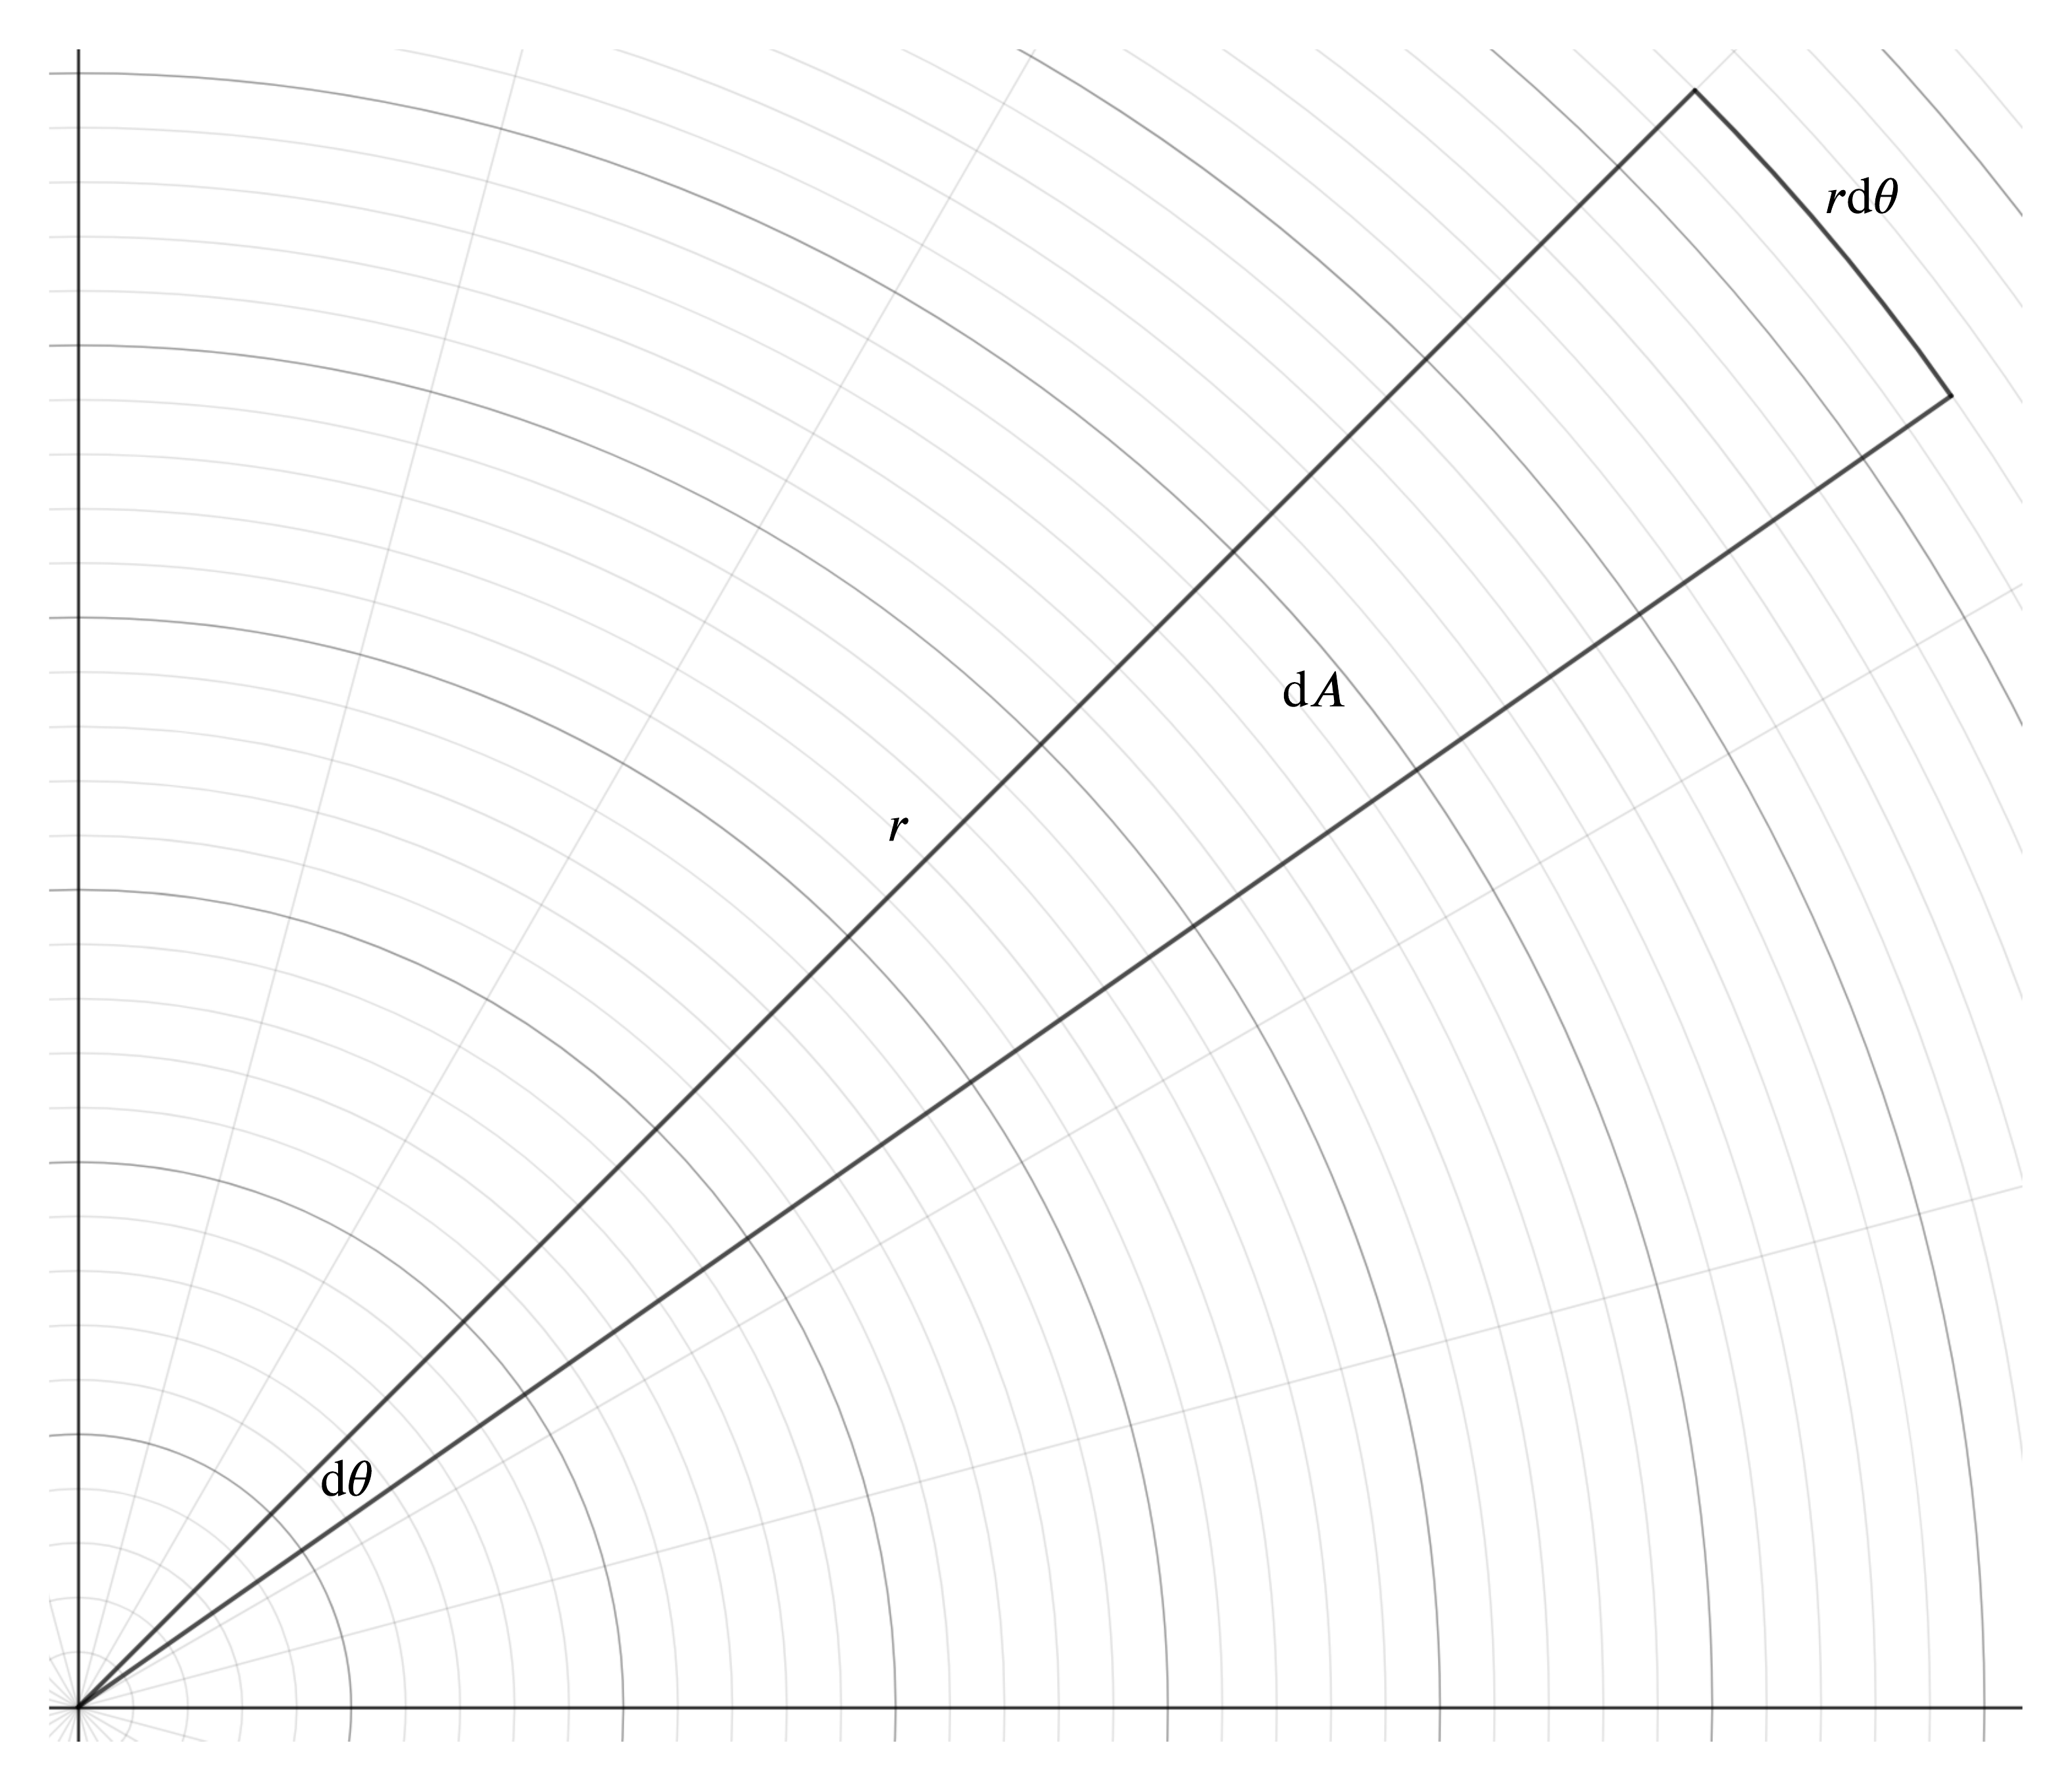
\includegraphics[width=0.66\textwidth]{./parametric_vector_polar/polar_area.png}
	\caption{\hyperref{}{}{}{Polar Area}}
\end{figure}

This circular sector has area $\d{A} = \frac{\d{\theta}}{2}r^2$.
Integrating $\d{A}$ for $\alpha \leq \theta \leq \beta$,
\begin{equation*}
	A = \int_{\alpha}^{\beta}{\frac{1}{2}r^2\d{\theta}} = \int_{\alpha}^{\beta}{\frac{1}{2}f^2(\theta)\d{\theta}}.
\end{equation*}

\begin{example}
	Find the area inside the smaller loop of the lima\c{c}on $r=2\cos{\theta}+1$.
\end{example}
\begin{answer}
	First, we need to find our bounds on $\theta$.
	We know that the small loop begins and ends when $r=0$.
	\begin{align*}
		0 &= 2\cos{\theta}+1 \\
		-\frac{1}{2} &= \cos{\theta} \\
		\theta &= \frac{\pi}{3}, \frac{4\pi}{3}.
	\end{align*}
	
	Now that we have our bounds, we can integrate.
	\begin{align*}
		A &= \int_{2\pi/3}^{4\pi/3}{\frac{1}{2}\left(2\cos{\theta}+1\right)^2\d{\theta}} \\
		&= \frac{1}{2}\left(\int_{\frac{2\pi}{3}}^{\frac{4\pi}{3}}4\cos^{2}\left(\theta\right)\d{\theta}+4\int_{\frac{2\pi}{3}}^{\frac{4\pi}{3}}\cos\left(\theta\right)\d{\theta}+\int_{\frac{2\pi}{3}}^{\frac{4\pi}{3}}\d{\theta}\right) \\
		&= \int_{\frac{2\pi}{3}}^{\frac{4\pi}{3}}\left(1+\cos\left(2\theta\right)\right)\d{\theta}+2\int_{\frac{2\pi}{3}}^{\frac{4\pi}{3}}\cos\left(\theta\right)\d{\theta}+\frac{1}{2}\int_{\frac{2\pi}{3}}^{\frac{4\pi}{3}}\d{\theta} \\
		&= \int_{\frac{2\pi}{3}}^{\frac{4\pi}{3}}\cos\left(2\theta\right)\d{\theta}+2\int_{\frac{2\pi}{3}}^{\frac{4\pi}{3}}\cos\left(\theta\right)\d{\theta}+\frac{3}{2}\int_{\frac{2\pi}{3}}^{\frac{4\pi}{3}}\d{\theta} \\
		&= \frac{1}{2}\sin\left(2\theta\right)+2\sin\left(\theta\right)+\frac{3}{2}\theta \biggr\rvert_{2\pi/3}^{4\pi/3} \\
		&= \left(\frac{1}{2}\sin\left(\frac{8\pi}{3}\right)+2\sin\left(\frac{4\pi}{3}\right)+\frac{3}{2}\frac{4\pi}{3}\right)-\left(\frac{1}{2}\sin\left(\frac{4\pi}{3}\right)+2\sin\left(\frac{2\pi}{3}\right)+\frac{3}{2}\frac{2\pi}{3}\right) \\
		&= \left(\frac{\sqrt{3}}{4}-\sqrt{3}+2\pi\right)-\left(-\frac{\sqrt{3}}{4}+\sqrt{3}+\pi\right) \\
		&= \frac{\sqrt{3}}{2}-2\sqrt{3}+\pi \\
		&= \pi-\frac{3\sqrt{3}}{2}.
	\end{align*}
\end{answer}

\subsubsection{Area Between Curves}
The area between $r_1(\theta)$ and $r_2(\theta)$ is simply the difference between the areas.
\begin{equation*}
	A = \frac{1}{2}\int_{\alpha}^{\beta}{r_1^2(\theta)\d{\theta}} - \frac{1}{2}\int_{\alpha}^{\beta}{r_2^2(\theta)\d{\theta}} = \frac{1}{2}\int_{\alpha}^{\beta}{(r_1^2(\theta)-r_2^2(\theta))\d{\theta}}.
\end{equation*}

\begin{example}
	Find the area that lies inside the circle $r=1$ and outside the cardioid $r=1-\cos{\theta}$.
\end{example}
\begin{answer}
	To find the bounds, we need to find where these curves intersect.
	\begin{align*}
		1 &= 1-\cos{\theta} \\
		\cos{\theta} &= 0 \\
		\theta &= \frac{\pi}{2}, \frac{-\pi}{2}.
	\end{align*}
	
	Since we want the area inside of the circle and outside of the cardioid, our bounds are $\frac{-\pi}{2} \leq \theta \leq \frac{\pi}{2}$.
	We'll also have $r_1(\theta)$ be the circle and $r_2(\theta)$ be the cardioid, since we are effectively finding the area inside the circle and subtracting away the area that is also in the cardioid.
	\begin{align*}
		A &= \frac{1}{2}\int_{-\pi/2}^{\pi/2}{\left(1^2 - \left(1-\cos{\theta}\right)^2\right)\d{\theta}} \\
		&= \frac{1}{2}\int_{\frac{-\pi}{2}}^{\frac{\pi}{2}}\left(2\cos\left(\theta\right)-\cos^{2}\theta\right)\d{\theta} \\
		&= \frac{1}{2}\int_{\frac{-\pi}{2}}^{\frac{\pi}{2}}\left(2\cos\left(\theta\right)-\frac{1+\cos\left(2\theta\right)}{2}\right)\d{\theta} \\
		&= \frac{1}{2}\left(2\sin\left(\theta\right)-\frac{\theta}{2}-\frac{\sin\left(2\theta\right)}{4}\right) \biggr\rvert_{\frac{-\pi}{2}}^{\frac{\pi}{2}} \\
		&= \frac{1}{2}\left(\left(2\sin\left(\frac{\pi}{2}\right)-\frac{\pi}{4}-\frac{\sin\left(\pi\right)}{4}\right)-\left(2\sin\left(\frac{-\pi}{2}\right)+\frac{\pi}{4}-\frac{\sin\left(-\pi\right)}{4}\right)\right) \\
		&= \left(2\sin\left(\frac{\pi}{2}\right)-\frac{\pi}{4}-\frac{\sin\left(\pi\right)}{4}\right) \\
		&= 2-\frac{\pi}{4}.
	\end{align*}
\end{answer}

\begin{example}
	Find the area that lies outside the circle $r=1$ and inside the cardioid $r=1-\cos{\theta}$.
\end{example}
\begin{answer}
	We need to make sure our bounds are sweeping out the correct area.
	If we did $\frac{-\pi}{2} \leq \theta \leq \frac{\pi}{2}$, we'd get the area inside the circle and outside the cardioid, which isn't what we want here.
	We know that for polar coordinates, $\frac{-\pi}{2} \equiv \frac{3\pi}{2}$.
	So, out bounds are $\frac{\pi}{2} \leq \theta \leq \frac{3\pi}{2}$.
	Since we want the area inside the cardioid and outside the circle, effectively taking the cardioid and subtracting away the intersection, so $r_1(\theta)$ is the cardioid, and $r_2(\theta)$ is the circle.
	\begin{align*}
		A &= \frac{1}{2}\int_{\pi/2}^{3\pi/2}{\left(\left(1-\cos{\theta}\right)^2-1^2\right)\d{\theta}} \\
		&= \frac{1}{2}\int_{\frac{\pi}{2}}^{\frac{3\pi}{2}}\left(\cos^{2}\left(\theta\right)-2\cos\left(\theta\right)\right)\d{\theta} \\
		&= \frac{1}{2}\int_{\frac{\pi}{2}}^{\frac{3\pi}{2}}\left(\frac{1+\cos\left(2\theta\right)}{2}-2\cos\left(\theta\right)\right)\d{\theta} \\
		&= \frac{1}{2}\left(\frac{\theta}{2}+\frac{\sin\left(2\theta\right)}{4}-2\sin\left(\theta\right)\right)\biggr\rvert_{\pi/2}^{3\pi/2} \\
		&= \frac{1}{2}\left(\left(\frac{3\pi}{4}+\frac{\sin\left(3\pi\right)}{4}-2\sin\left(\frac{3\pi}{2}\right)\right)-\left(\frac{\pi}{4}+\frac{\sin\left(\pi\right)}{4}-2\sin\left(\frac{\pi}{2}\right)\right)\right) \\
		&= \frac{\pi}{4}+2.
	\end{align*}
\end{answer}

\begin{example}
	Find the area inside both the circle $r=1$ and the cardioid $r=1-\cos{\theta}$.
\end{example}
\begin{answer}
	This area isn't between two polar curves like the previous examples in the sense that we can't define it as one region minus another.
	We'll prove it it two ways: logically and by using two regions.
	Logically, we know that the total area of the circle is $\pi$.
	We also know the area inside the circle but outside the cardioid is $2-\frac{\pi}{4}$.
	So,
	\begin{equation*}
		A_{\text{both}} = \pi - \left(2-\frac{\pi}{4}\right) = \frac{5\pi}{4} - 2.
	\end{equation*}
	
	We can break the region inside both curves into two parts: a half circle for $x\leq 0$ and the two cardioid bulges for $x\geq 0$.
	The area of the half-circle is $\pi/2$.
	We can find the area of the two cardioid bulges.
	\begin{align*}
		A_{\text{bulges}} &= 2A_{\text{bulge}} \\
		&= \int_{0}^{\pi/2}{\left(1-\cos{\theta}\right)^2\d{\theta}} \\
		&= \int_{0}^{\frac{\pi}{2}}\left(\cos^{2}\theta-2\cos\left(\theta\right)+1\right)\d{\theta} \\
		&= \int_{0}^{\frac{\pi}{2}}\left(\frac{1+\cos\left(2\theta\right)}{2}-2\cos\left(\theta\right)+1\right)\d{\theta} \\
		&= \frac{3\theta}{2}+\frac{\sin\left(2\theta\right)}{4}-2\sin\left(\theta\right)\biggr\rvert_{0}^{\frac{\pi}{2}} \\
		&= \frac{3\pi}{4}+\frac{\sin\left(\pi\right)}{4}-2\sin\left(\frac{\pi}{2}\right) \\
		&= \frac{3\pi}{4}-2 \\
	\end{align*}
	
	Adding in the area of the half-circle,
	\begin{align*}
		A_{\text{both}} &= A_{\text{half}} + A_{\text{bulges}} \\
		&= \frac{\pi}{2} + \frac{3\pi}{4} - 2 \\
		&= \frac{5\pi}{4} - 2.
	\end{align*}
	
	We see that we get the same answer either way.
\end{answer}

\subsubsection{Arc Length}
Since we know how to convert polar functions to parametric, we can simply adapt the parametric arc length formula.
\begin{equation*}
	s = \int_{\alpha}^{\beta}{\sqrt{\left(\dd{x}{\theta}\right)^2 + \left(\dd{y}{\theta}\right)^2}\d{\theta}}.
\end{equation*}


However, there is an alternate form that works just for polar functions.
For some small change $\d{\theta}$, we see a corresponding small changes $\d{r}$ and $r\d{\theta}$.
\begin{figure}[H]
	\label{polar_area}
	\centering
	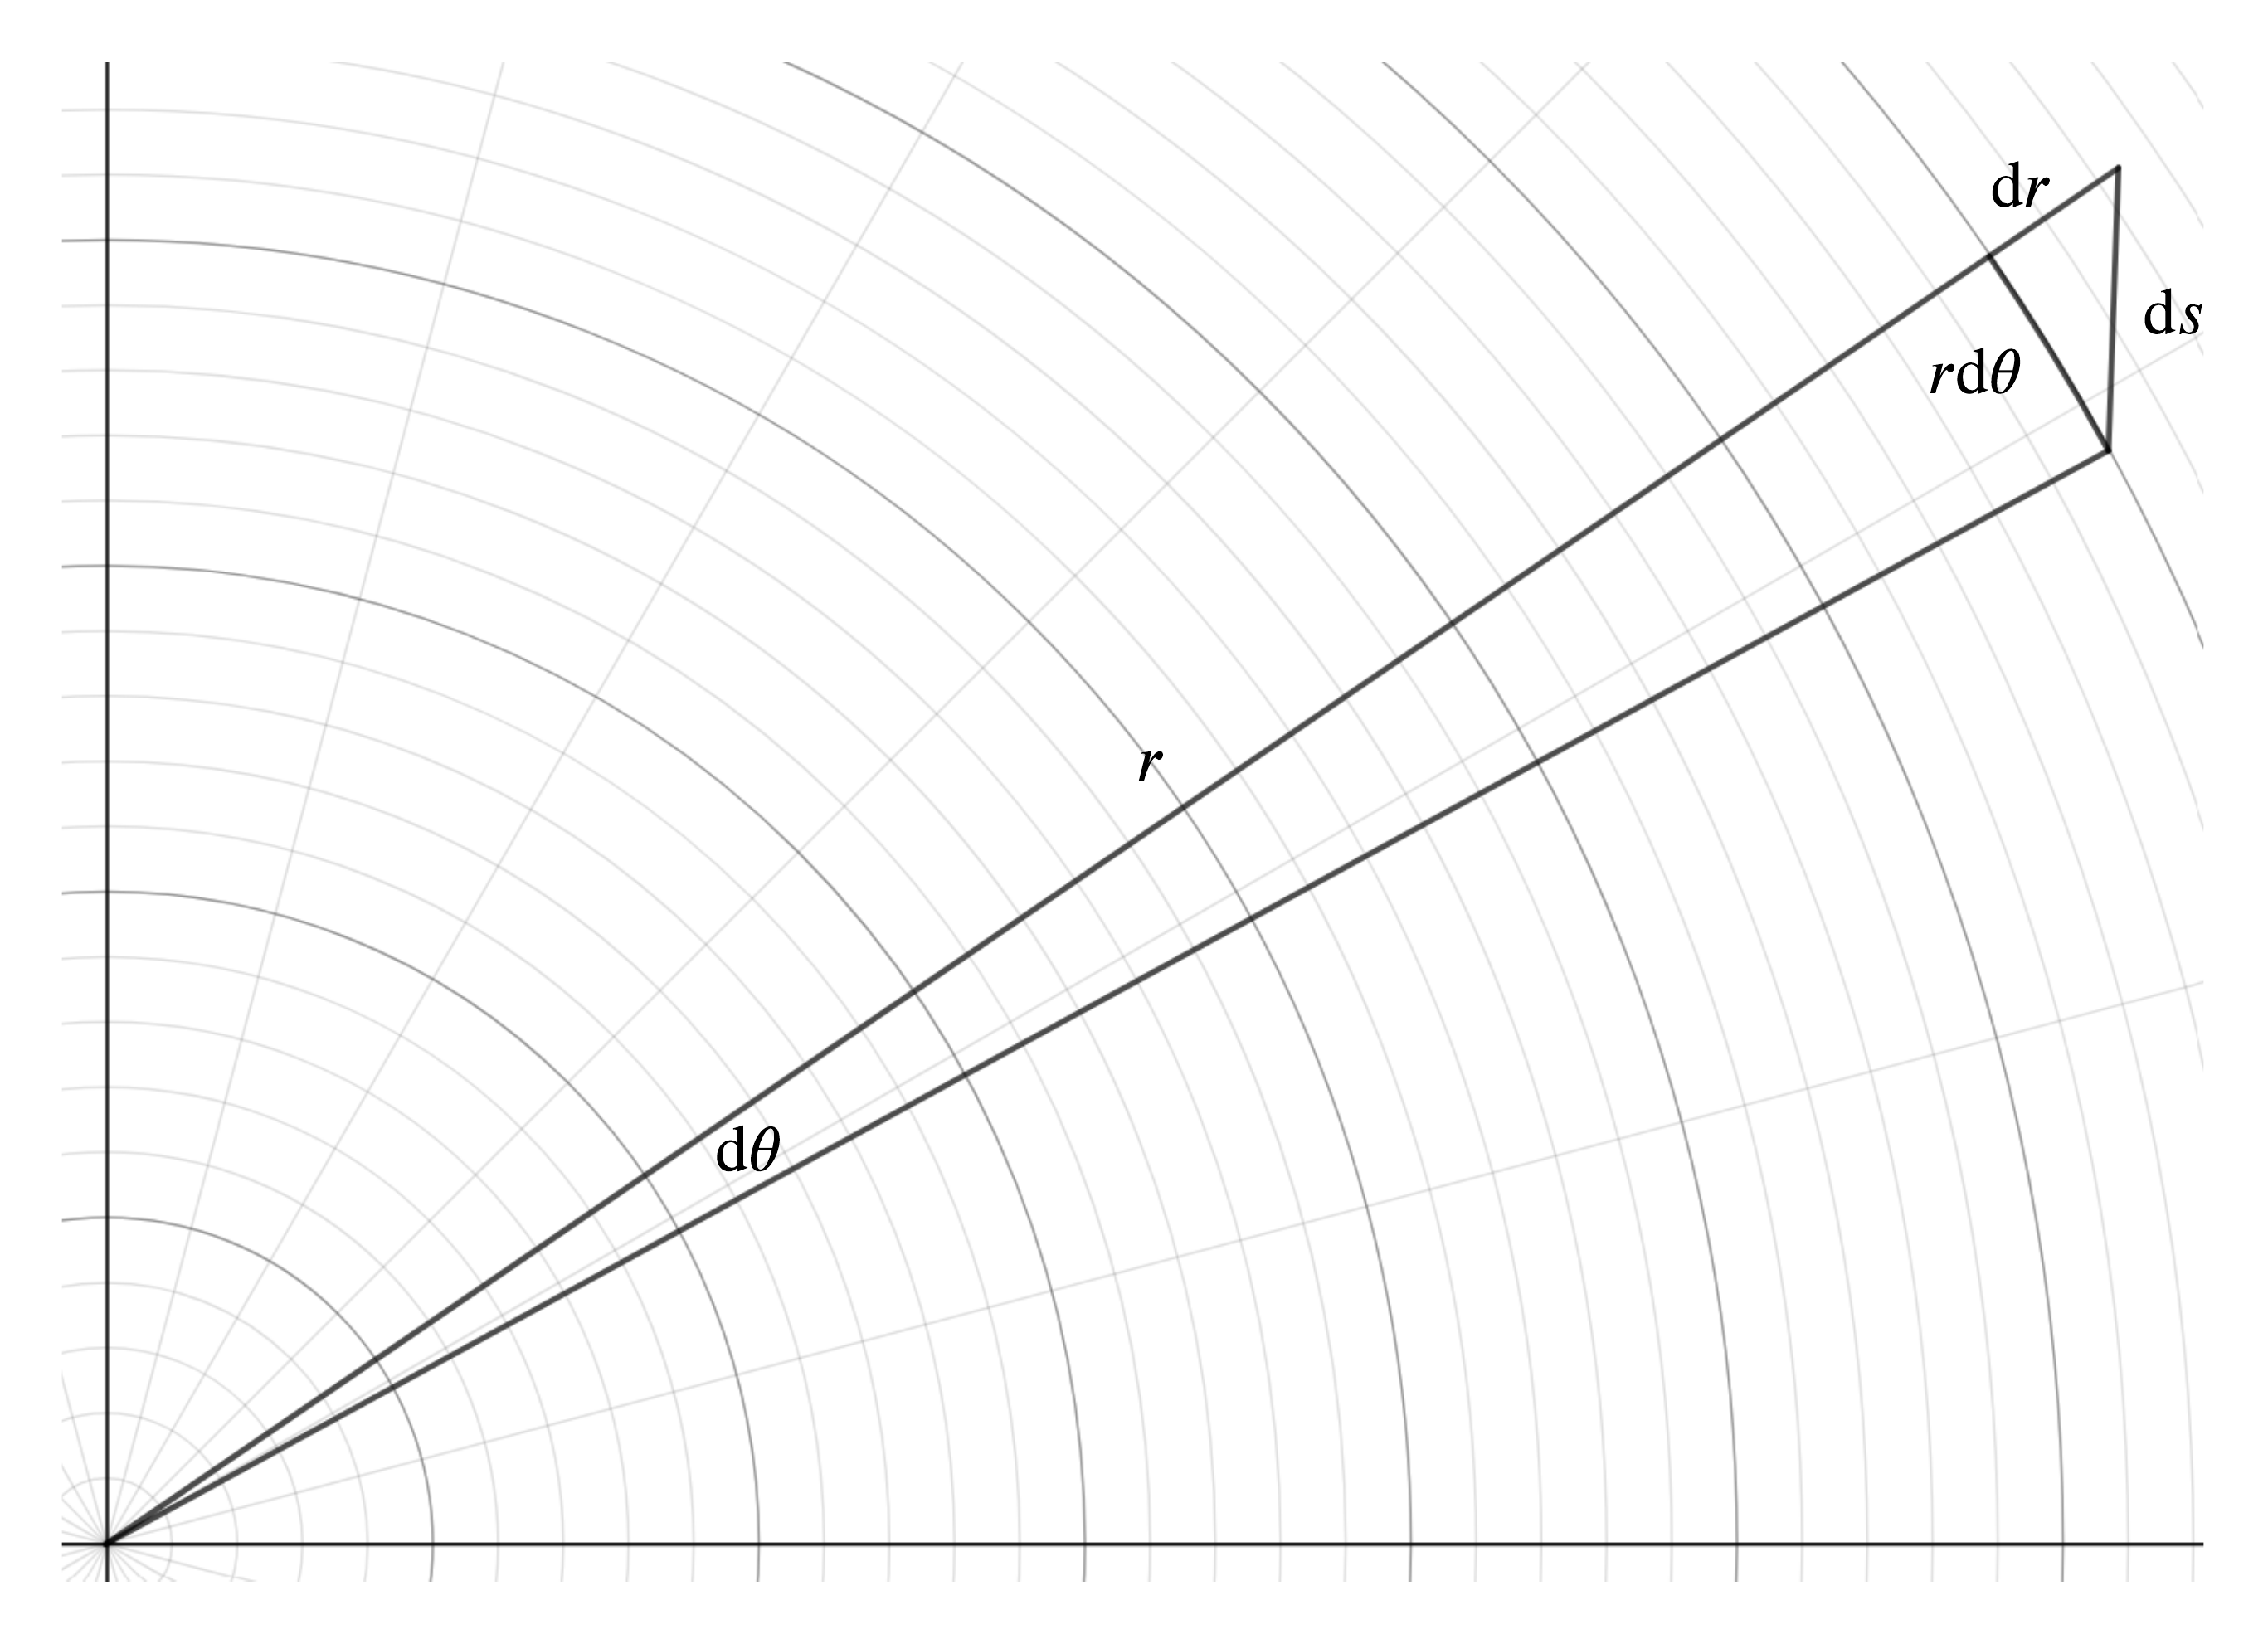
\includegraphics[width=0.66\textwidth]{./parametric_vector_polar/polar_length.png}
	\caption{\hyperref{}{}{}{Polar Arc Length}}
\end{figure}
We see that these changes for a right triangle with hypotenuse $\d{s}$.
\begin{align*}
	(\d{s})^2 &= (r\d{\theta})^2 + (\d{r})^2 \\
	&= \left(r^2 + \left(\dd{r}{\theta}\right)^2\right)\left(\d{\theta}\right)^2 \\
	\d{s} &= \sqrt{r^2 + \left(\dd{r}{\theta}\right)^2}\d{\theta} \\
	s &= \int_{\alpha}^{\beta}{\sqrt{r^2 + \left(\dd{r}{\theta}\right)^2}\d{\theta}}.
\end{align*}

Giving us an alternate formula for polar arc length.

\begin{example}
	Find the arc length of the cardioid $r=1-\cos{\theta}$.
\end{example}
\begin{answer}
	The bounds are $0 \leq \theta \leq 2\pi$.
	Using the polar arc length formula,
	\begin{align*}
		\dd{r}{\theta} &= \sin{\theta} \\
		\left(\dd{r}{\theta}\right)^2 &= \sin^2{\theta} \\
		s &= \int_{0}^{2\pi}{\sqrt{\left(1-\cos{\theta}\right)^2+\sin^2{\theta}}\d{\theta}} \\
		&= \int_{0}^{2\pi}{\sqrt{2+2\cos{\theta}}\d{\theta}} \\
		&= \int_{0}^{2\pi}{2\sin{\left(\frac{\theta}{2}\right)}\d{\theta}} \\
		&= -4\cos{\left(\frac{\theta}{2}\right)}\biggr\rvert_{0}^{2\pi} \\
		&= 8.
	\end{align*}
\end{answer}
